\chapter{Results}
\label{sec:results}

%FLOATING POTENTIAL SUMMARY
% \begin{table}[]
% \centering
% \begin{tabular}{cccccc}
% \hline
% & No photoelectron & Drift along Z & Drift along X & External Magnetic Field & Photoelectron temperature 3 eV\\\hline
% With booms & N/A & 105.419 & 105.400 & 105.400 & 78.154\\\hline
% Without booms & N/A & 100.710 & 100.696 & 100.699 & N/A\\\hline
% \end{tabular}
% \caption{Dummy text}
% \label{tab:FlotingPotSummary}
% \end{table}

\section{Charging without photoemission}
%FLOATING POTENTIAL CONVERGENCE
\begin{center}
    \begin{figure}[H]
      \begin{subfigure}[b]{0.75\textwidth}
      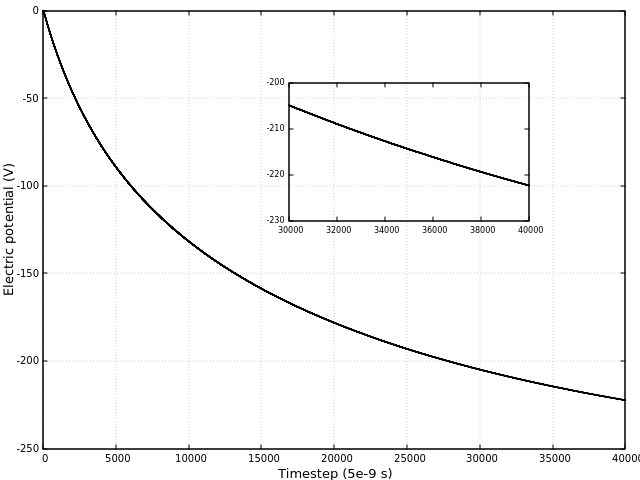
\includegraphics[width=\columnwidth]{figures/MMO/noPH/WB/C_noPH_WB.png}
      \caption{Booms}
      \label{fig:C_noPH_WB}
    \end{subfigure}
    \par\bigskip
    \begin{subfigure}[b]{0.75\textwidth}
      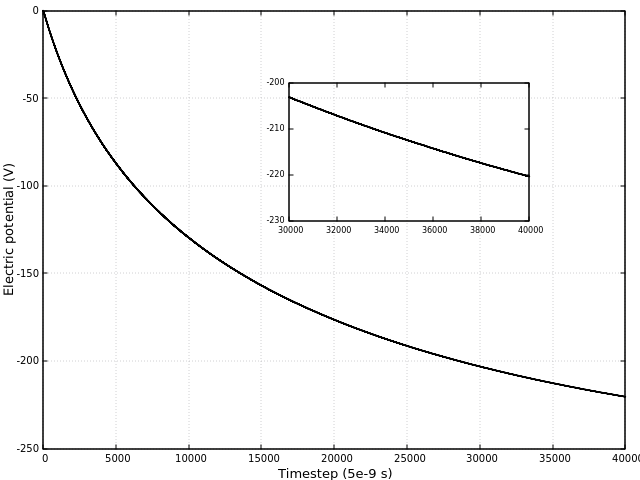
\includegraphics[width=\columnwidth]{figures/MMO/noPH/NB/C_noPH_NB.png}
      \caption{Without booms}
      \label{fig:C_noPH_NB}
    \end{subfigure}
  \label{fig:ConvnoPH}
  \caption{Timeseries plot of potential of the MMO with and without booms. The potential has been converted from PINC dimensionless units to Volts. The inset plots shows the potential of the two configurations for last 10,000 timesteps.}
  \end{figure}
\end{center}

%POTENTIAL THROUGH CENTER OF OBJECT
\begin{center}
    \begin{figure}[H]
      \begin{subfigure}[b]{0.61\textwidth}
      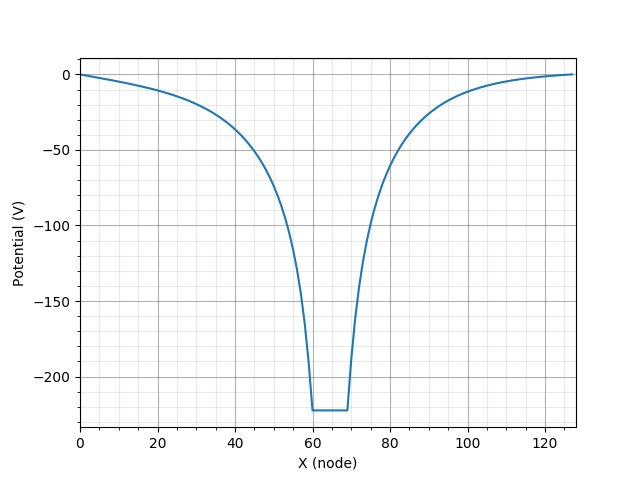
\includegraphics[width=\textwidth]{figures/MMO/noPH/WB/L_noPH_WB.png}
      \caption{Booms}
      \label{fig:L_noPH_WB}
    \end{subfigure}
    \begin{subfigure}[b]{0.61\textwidth}
      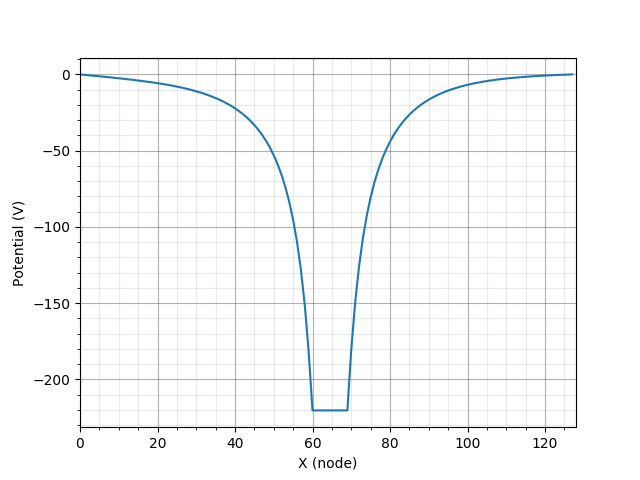
\includegraphics[width=\textwidth]{figures/MMO/noPH/NB/L_noPH_NB.png}
      \caption{Without booms}
      \label{fig:L_noPH_NB}
    \end{subfigure}
  \label{fig:Line_noPH}
  \caption{\ref{fig:L_noPH_NB} and \ref{fig:L_noPH_WB} show a potential profile along the X axis for the MMO without and with booms respectively. The line is plotted at $(x,y) = (13.95 m, 13.95 m)$, or node points $(x,y) = (62,62)$, and passes through the main octagonal body of the spacecraft. The X axis units are in number of nodes from the origin.}
  \end{figure}
\end{center}

%AVERAGE POTENTIAL ISOLINES XY
\begin{center}
\begin{figure}[H]
  \begin{subfigure}[b]{0.61\textwidth}
    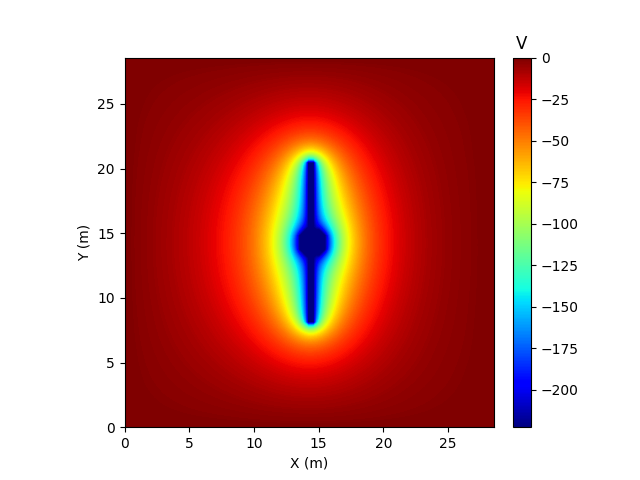
\includegraphics[width=\textwidth]{figures/MMO/noPH/WB/P_noPH_WB.png}
    \caption{Booms}
    \label{fig:P_noPH_WB}
  \end{subfigure}
  \hfill
  \begin{subfigure}[b]{0.61\textwidth}
    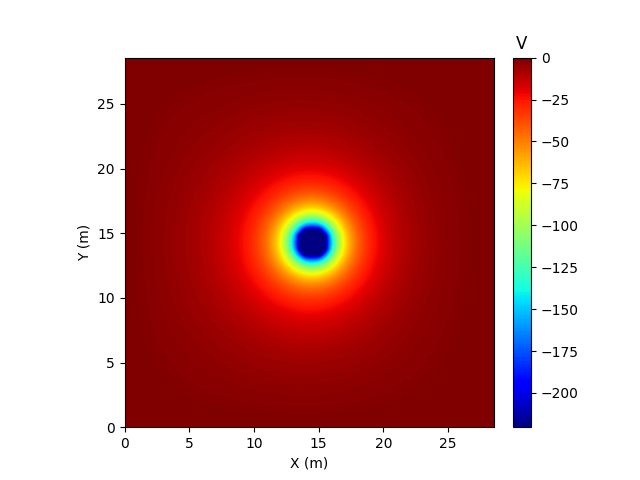
\includegraphics[width=\textwidth]{figures/MMO/noPH/NB/P_noPH_NB.png}
    \caption{Without booms}
    \label{fig:P_noPH_NB}
  \end{subfigure}
  \label{fig:Pot_noPH}
  \caption{\ref{fig:P_noPH_WB} and \ref{fig:P_noPH_WB} are 2D slice through $Z = 14.4 m$ showing the potential profile of the entire computational domain.}
\end{figure}
\end{center}

%PARTICLE DENSITIES (rho_i and rho_e)
%RHO_I
\begin{center}
    \begin{figure}[H]
      \begin{subfigure}[b]{0.61\textwidth}
      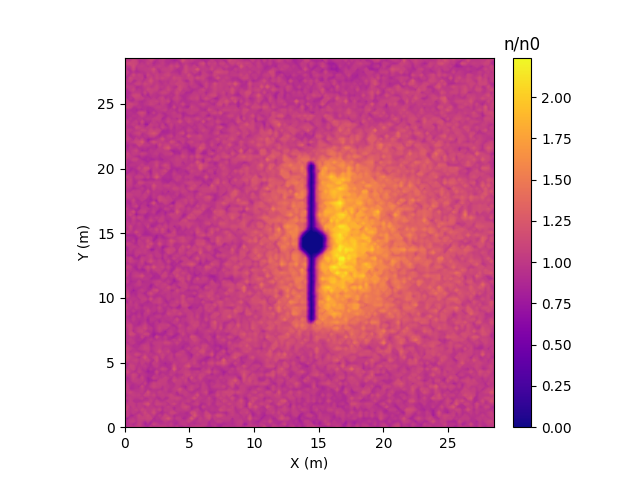
\includegraphics[width=\textwidth]{figures/MMO/noPH/WB/I_noPH_WB.png}
      \caption{Booms}
      \label{fig:I_noPH_WB}
    \end{subfigure}
    \begin{subfigure}[b]{0.61\textwidth}
      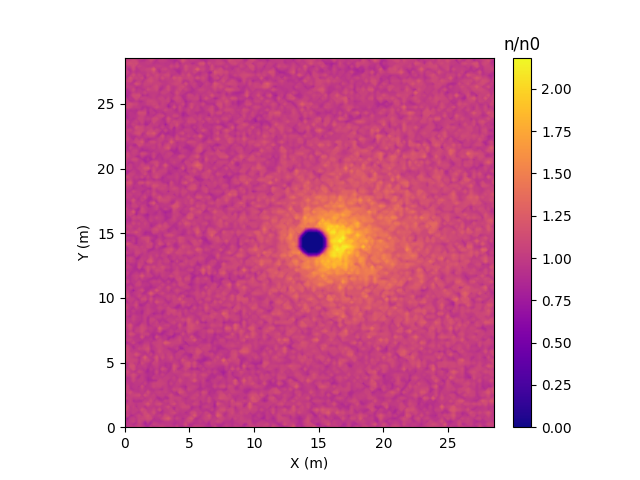
\includegraphics[width=\textwidth]{figures/MMO/noPH/NB/I_noPH_NB.png}
      \caption{Without booms}
      \label{fig:I_noPH_NB}
    \end{subfigure}
  \label{fig:Ions_noPH}
  \caption{Ion density profile plotted at $Z = 14.4 m$, the color gradient is normalized against the ion plasma density from table \ref{tab:PlasmaParamMMO}.}
  \end{figure}
\end{center}

%RHO_E
\begin{center}
    \begin{figure}[H]
      \begin{subfigure}[b]{0.61\textwidth}
      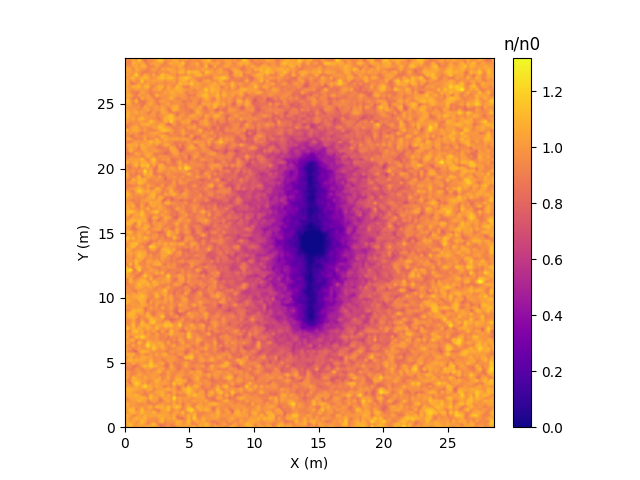
\includegraphics[width=\textwidth]{figures/MMO/noPH/WB/E_noPH_WB.png}
      \caption{Booms}
      \label{fig:E_noPH_WB}
    \end{subfigure}
    \begin{subfigure}[b]{0.61\textwidth}
      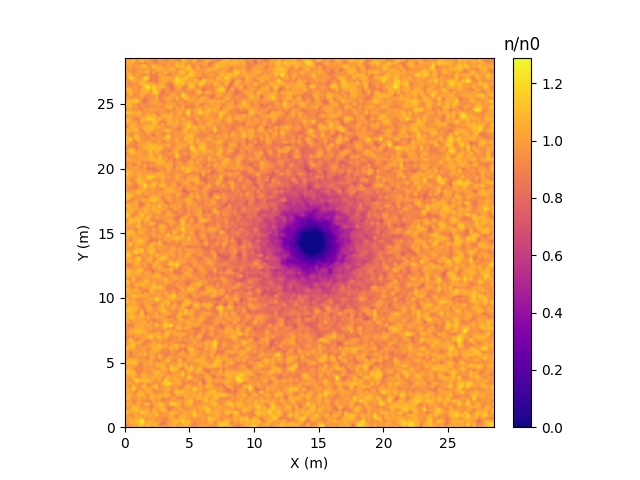
\includegraphics[width=\textwidth]{figures/MMO/noPH/NB/E_noPH_NB.png}
      \caption{Without booms}
      \label{fig:E_noPH_NB}
    \end{subfigure}
  \label{fig:Elec_noPH}
  \caption{Electron density profile plotted at $Z = 14.4 m$, the color gradient is normalized against the electron plasma density from table \ref{tab:PlasmaParamMMO}.}
  \end{figure}
\end{center}


\section{Charging with photoemission}

\subsection*{Drift parallel to X axis}

%FLOATING POTENTIAL CONVERGENCE
\begin{figure}[H]
  \centering
  \begin{subfigure}[b]{0.75\textwidth}
  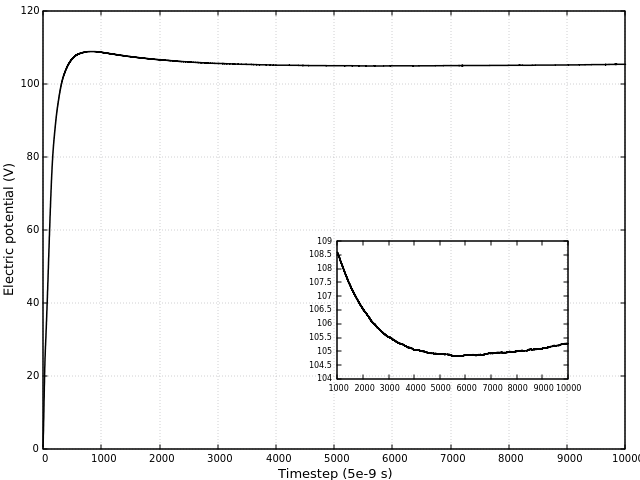
\includegraphics[width=\columnwidth]{figures/MMO/posX/WB/C_posX_WB.png}
  \caption{Booms}
  \label{fig:C_posX_WB}
\end{subfigure}
\hfill
\begin{subfigure}[b]{0.75\textwidth}
  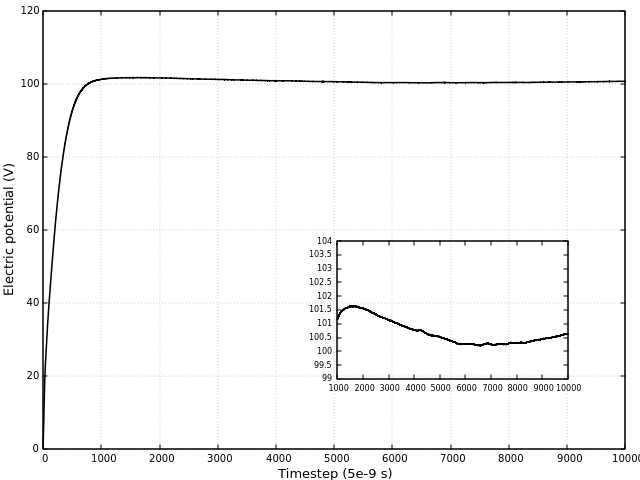
\includegraphics[width=\columnwidth]{figures/MMO/posX/NB/C_posX_NB.png}
  \caption{Without booms}
  \label{fig:C_posX_NB}
\end{subfigure}
\label{fig:Conv_posX}
\caption{Time series plot of the potential of the two MMO configurations for drift along X axis. The insets plots the same timeseries starting at 1000 timesteps, where the potential of the spacecraft has begun to oscillate about the floating potential.}
\end{figure}


%POTENTIAL THROUGH CENTER OF OBJECT

\begin{figure}[H]
  \begin{subfigure}[b]{0.6\textwidth}
  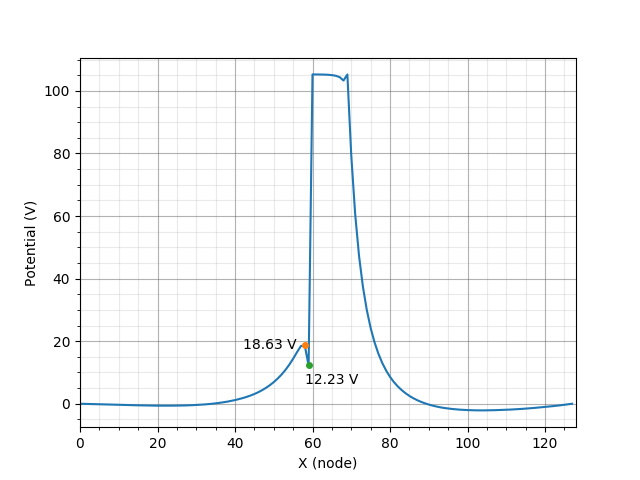
\includegraphics[width=\textwidth]{figures/MMO/posX/WB/L_posX_WB.png}
  \caption{Booms}
  \label{fig:L_posX_WB}
\end{subfigure}
\begin{subfigure}[b]{0.6\textwidth}
  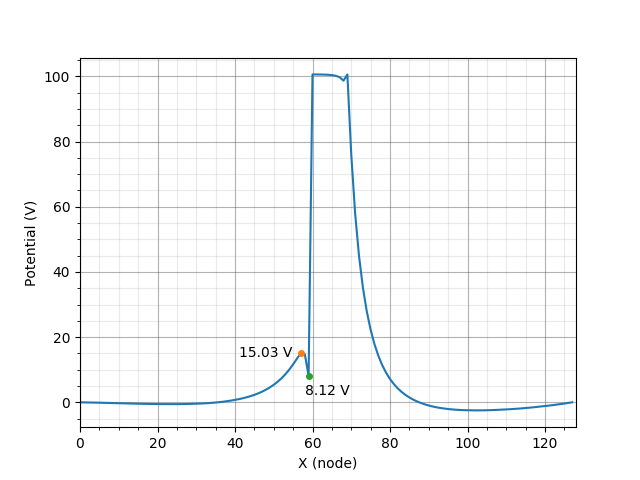
\includegraphics[width=\textwidth]{figures/MMO/posX/NB/L_posX_NB.png}
  \caption{Without booms}
  \label{fig:L_posX_NB}
\end{subfigure}
\label{fig:Line_posX}
\caption{Potential profile along the X axis for the two MMO configurations with drift along the X axis and photoemission included. The line is plotted at $(x,y) = (13.95 m, 13.95 m)$, or node points $(x,y) = (62,62)$, and passes through the main octagonal body of the spacecraft. The X axis units are in number of nodes from the origin. The two values in each plot show the height of the potential barrier formed.}
\end{figure}


%AVERAGE POTENTIAL ISOLINES XY

\begin{figure}[H]
  \begin{subfigure}[b]{0.6\textwidth}
    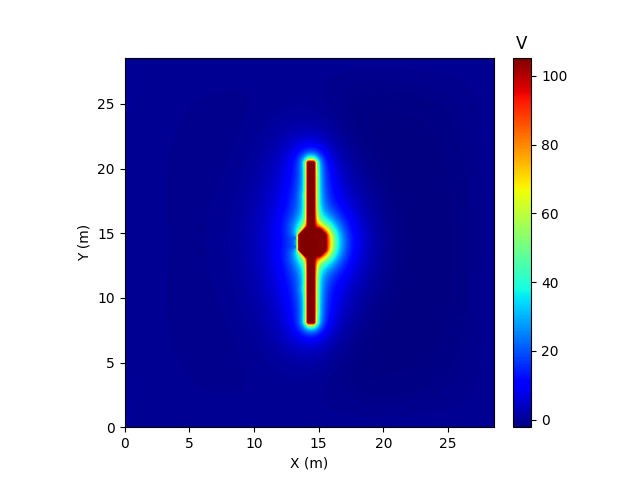
\includegraphics[width=\textwidth]{figures/MMO/posX/WB/P_posX_WB.png}
    \caption{Booms}
    \label{fig:P_posX_WB}
  \end{subfigure}
  \begin{subfigure}[b]{0.6\textwidth}
    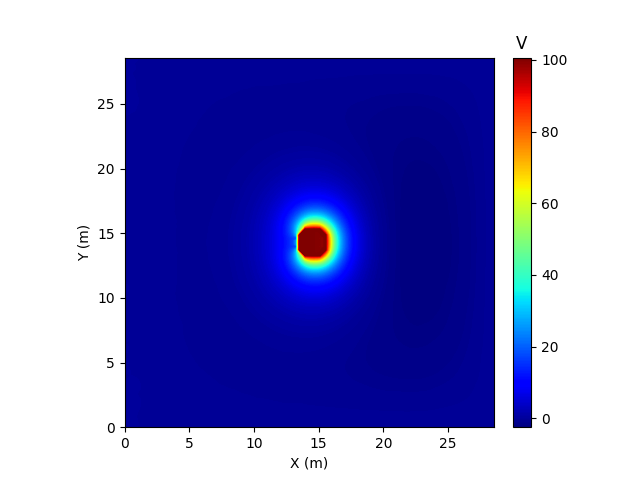
\includegraphics[width=\textwidth]{figures/MMO/posX/NB/P_posX_NB.png}
    \caption{Without booms}
    \label{fig:P_posX_NB}
  \end{subfigure}
  \label{fig:Pot_posX}
  \caption{2D slice through $Z = 14.4 m$ showing the time averaged potential profile of the entire computational domain with drift along X axis, and photoemission included. The potential is time averaged after a floating potential has been reached after 1,000 timesteps.}
\end{figure}



%PARTICLE DENSITIES (rho_i and rho_e)
%RHO_I

\begin{figure}[H]
  \begin{subfigure}[b]{0.6\textwidth}
  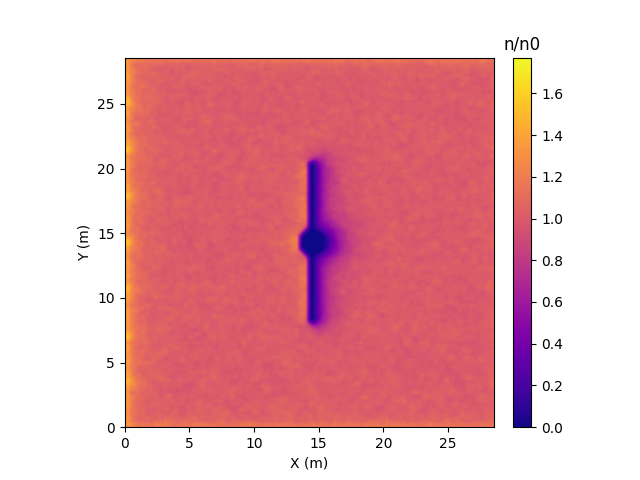
\includegraphics[width=\textwidth]{figures/MMO/posX/WB/I_posX_WB.png}
  \caption{Booms}
  \label{fig:I_posX_WB}
  \end{subfigure}
\begin{subfigure}[b]{0.6\textwidth}
  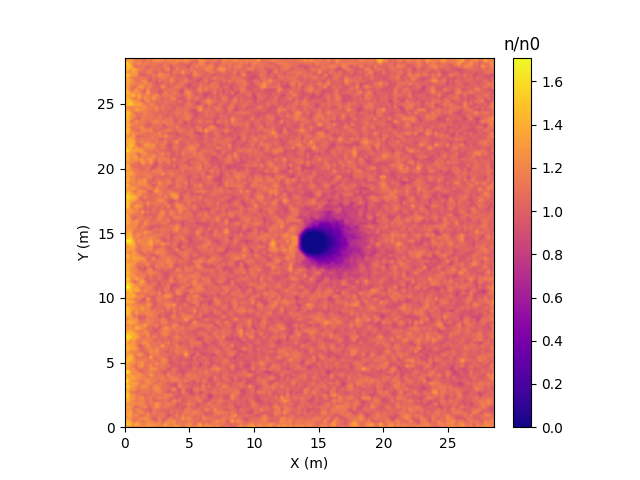
\includegraphics[width=\textwidth]{figures/MMO/posX/NB/I_posX_NB.png}
  \caption{Without booms}
  \label{fig:I_posX_NB}
\end{subfigure}
\label{fig:Ions_posX}
\caption{Ion density profile plotted at $Z = 14.4 m$, the color gradient is normalized against the ion plasma density from table \ref{tab:PlasmaParamMMO}. Plasma drift is along the X axis, and photoemission is included}
\end{figure}


%RHO_E

\begin{figure}[H]
  \begin{subfigure}[b]{0.6\textwidth}
  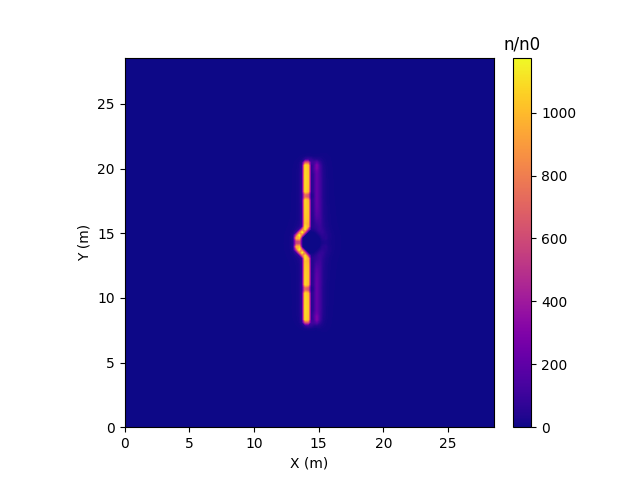
\includegraphics[width=\textwidth]{figures/MMO/posX/WB/E_posX_WB.png}
  \caption{Booms}
  \label{fig:E_posX_WB}
\end{subfigure}
\begin{subfigure}[b]{0.6\textwidth}
  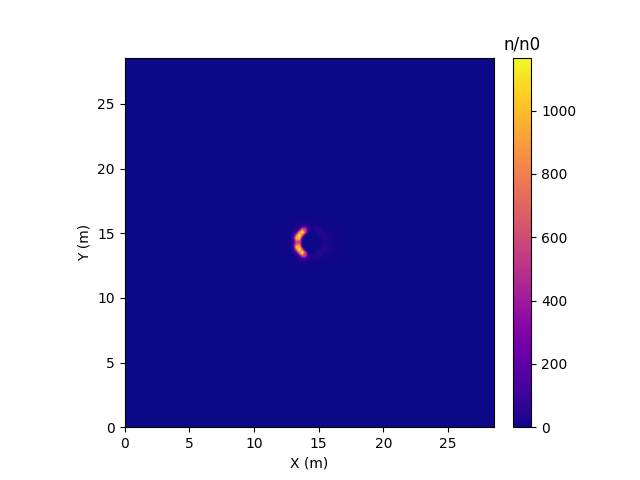
\includegraphics[width=\textwidth]{figures/MMO/posX/NB/E_posX_NB.png}
  \caption{Without booms}
  \label{fig:E_posX_NB}
\end{subfigure}
\label{fig:Elec_posX}
\caption{Electron density profile plotted at $Z = 14.4 m$, the color gradient is normalized against the electron plasma density from table \ref{tab:PlasmaParamMMO}. Drift is along the X axis, and photoemission is included, the sun is located in the negative X direction.}
\end{figure}




\subsection*{Drift parallel to Z axis}
%FLOATING POTENTIAL CONVERGENCE

\begin{figure}[H]
  \centering
  \begin{subfigure}[b]{0.75\textwidth}
  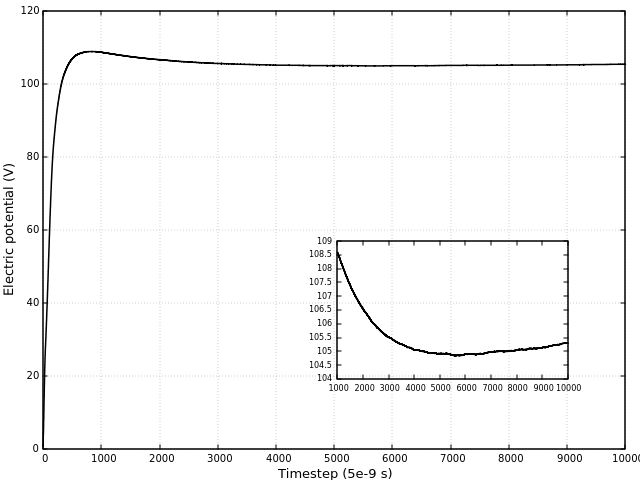
\includegraphics[width=\columnwidth]{figures/MMO/minZ/WB/C_minZ_WB.png}
  \caption{Booms}
  \label{fig:C_minZ_WB}
\end{subfigure}
\par\bigskip
\begin{subfigure}[b]{0.75\textwidth}
  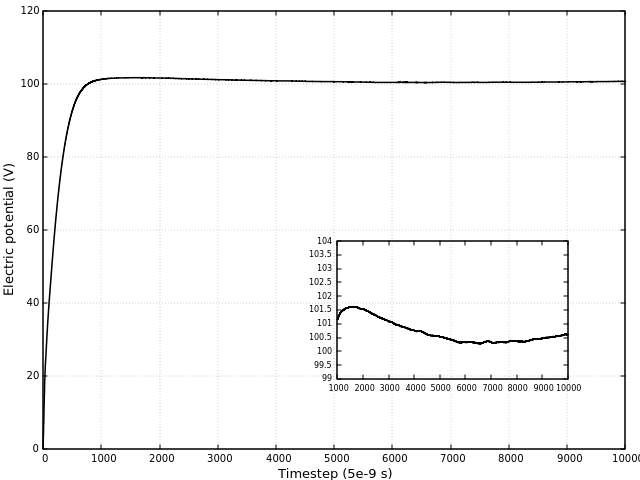
\includegraphics[width=\columnwidth]{figures/MMO/minZ/NB/C_minZ_NB.png}
  \caption{Without booms}
  \label{fig:C_minZ_NB}
\end{subfigure}
\label{fig:Conv_minZ}
\caption{Time series plot of the potential of the MMO with and without booms, where the drift is along the negative Z axis and photoemission is included. The inset plots the same timeseries after 1000 timesteps, where the potential of the spacecraft has begun to oscillate about the floating potential.}
\end{figure}


%POTENTIAL THROUGH CENTER OF OBJECT
\begin{figure}[H]
  \begin{subfigure}[b]{0.6\textwidth}
  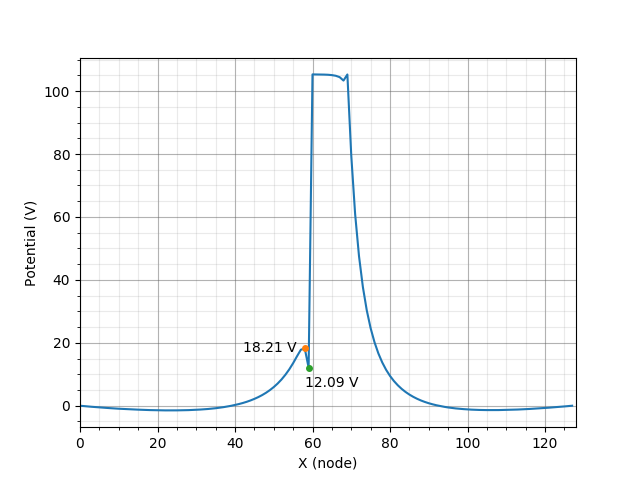
\includegraphics[width=\textwidth]{figures/MMO/minZ/WB/L_minZ_WB.png}
  \caption{Booms}
  \label{fig:L_minZ_WB}
\end{subfigure}
\begin{subfigure}[b]{0.6\textwidth}
  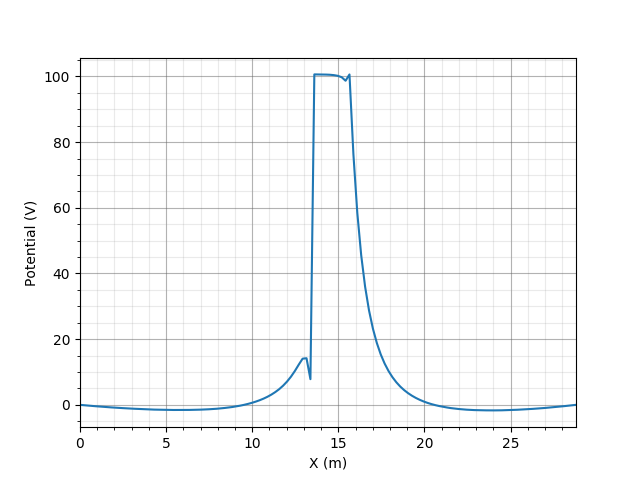
\includegraphics[width=\textwidth]{figures/MMO/minZ/NB/L_minZ_NB.png}
  \caption{Without booms}
  \label{fig:L_minZ_N}
\end{subfigure}
\label{fig:Line_minZ}
\caption{Potential profile along the X axis for the two MMO configurations with drift along the negative Z axis and photoemission included. The line is plotted at $(x,y) = (13.95 m, 13.95 m)$, or node points $(x,y) = (62,62)$, and passes through the main octagonal body of the spacecraft. The X axis units are in number of nodes from the origin. The two values in each plot show the height of the potential barrier formed.}
\end{figure}


%AVERAGE POTENTIAL ISOLINES XY
\begin{figure}[H]
  \begin{subfigure}[b]{0.6\textwidth}
    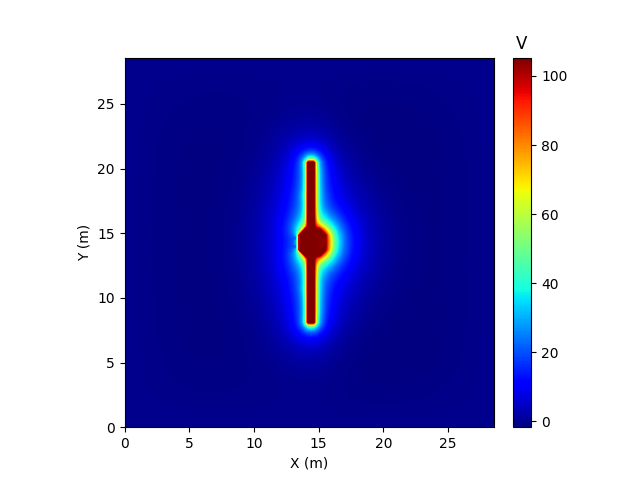
\includegraphics[width=\textwidth]{figures/MMO/minZ/WB/P_minZ_WB.png}
    \caption{Booms}
    \label{fig:P_minZ_WB}
  \end{subfigure}
  \hfill
  \begin{subfigure}[b]{0.6\textwidth}
    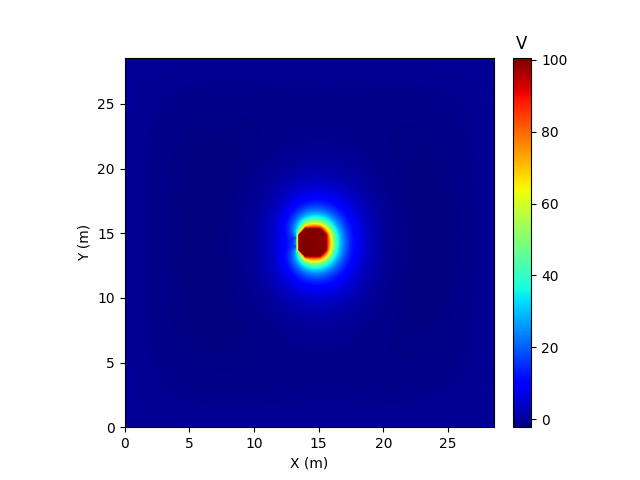
\includegraphics[width=\textwidth]{figures/MMO/minZ/NB/P_minZ_NB.png}
    \caption{Without booms}
    \label{fig:P_minZ_NB}
  \end{subfigure}
  \label{fig:Pot_minZ}
  \caption{2D slice through $Z = 14.4 m$ showing the time averaged potential profile of the entire computational domain with drift along the negative Z axis, and photoemission included. The potential is time averaged after a floating potential has been reached after 1,000 timesteps.}
\end{figure}

%PARTICLE DENSITIES (rho_i and rho_e)
%RHO_I
\begin{figure}[H]
  \begin{subfigure}[b]{0.6\textwidth}
  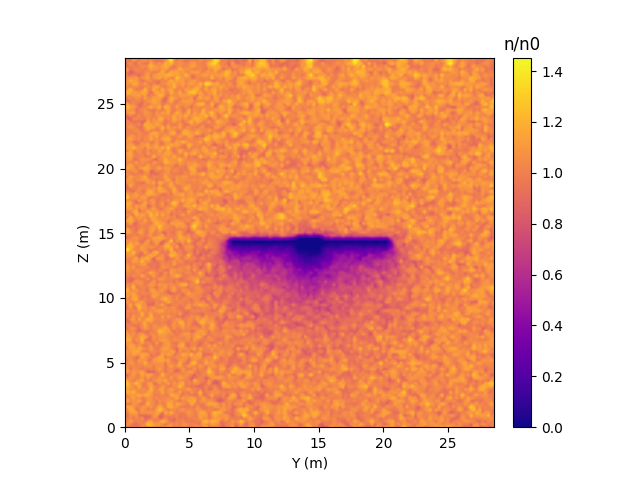
\includegraphics[width=\textwidth]{figures/MMO/minZ/WB/I_minZ_WB.png}
  \caption{Booms}
  \label{fig:I_minZ_WB}
\end{subfigure}
\begin{subfigure}[b]{0.6\textwidth}
  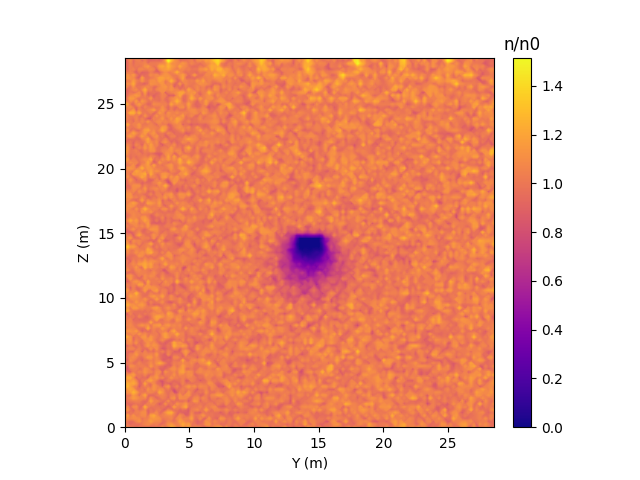
\includegraphics[width=\textwidth]{figures/MMO/minZ/NB/I_minZ_NB.png}
  \caption{Without booms}
  \label{fig:I_minZ_NB}
\end{subfigure}
\label{fig:Ion_minZ}
\caption{Ion density profile plotted at $Y = 14.4 m$, the color gradient is normalized against the ion plasma density from table \ref{tab:PlasmaParamMMO}. Drift is along the negative Z axis. and photoemission is included.}
\end{figure}

%RHO_E
\begin{figure}[H]
  \begin{subfigure}[b]{0.6\textwidth}
  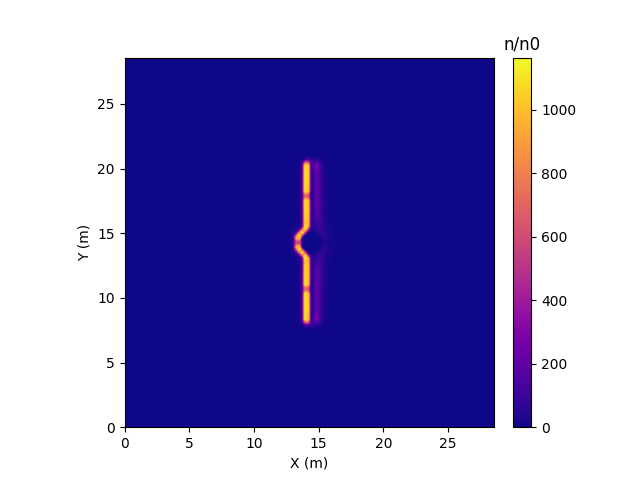
\includegraphics[width=\textwidth]{figures/MMO/minZ/WB/E_minZ_WB.png}
  \caption{Booms}
  \label{fig:E_minZ_WB}
\end{subfigure}
\begin{subfigure}[b]{0.6\textwidth}
  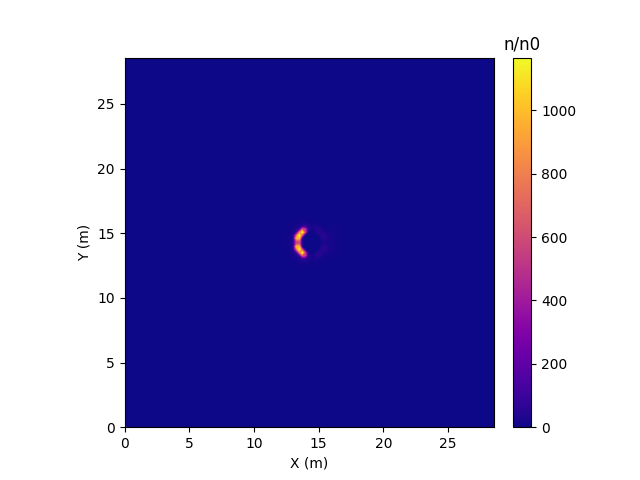
\includegraphics[width=\textwidth]{figures/MMO/minZ/NB/E_minZ_NB.png}
  \caption{Without booms}
  \label{fig:E_minZ_NB}
\end{subfigure}
\label{fig:Elec_minZ}
\caption{Electron density profile plotted at $Z = 14.4 m$, the color gradient is normalized against the electron plasma density from table \ref{tab:PlasmaParamMMO}. Drift is directed into the page, and photoemission is included. The sun is located in the negative X direction.}
\end{figure}


\section{Charging in an external magnetic field}

%FLOATING POTENTIAL CONVERGENCE
\begin{figure}[H]
  \begin{subfigure}[b]{0.75\textwidth}
  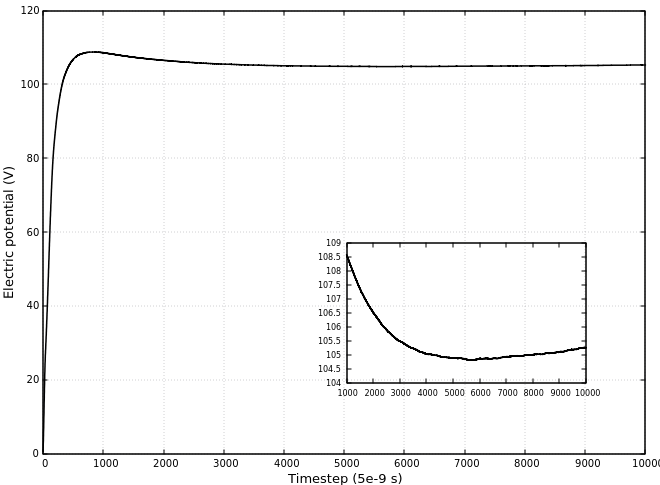
\includegraphics[width=\columnwidth]{figures/MMO/BField/WB/C_BField_WB.png}
  \caption{Booms}
  \label{fig:C_BField_WB}
\end{subfigure}
\par\bigskip
\begin{subfigure}[b]{0.75\textwidth}
  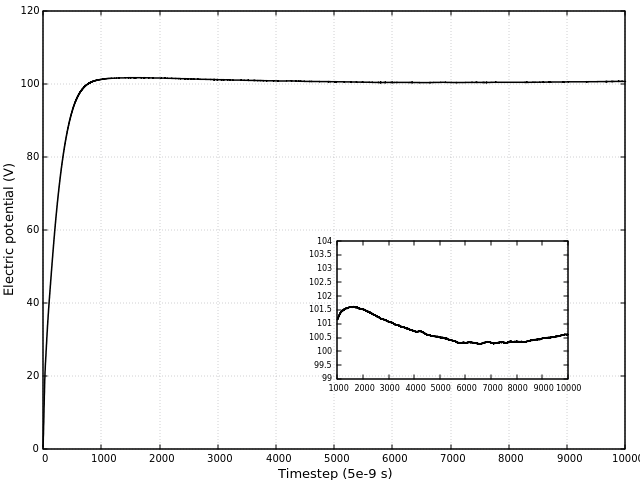
\includegraphics[width=\columnwidth]{figures/MMO/BField/NB/C_BField_NB.png}
  \caption{Without booms}
  \label{fig:C_BField_NB}
\end{subfigure}
\label{fig:Conv_BField}
\caption{Timeseries plot of the potential of the two configurations of the MMO, drift is along the negative Z axis, photoemission and an external magnetic field are included. The potential has been converted from PINC dimensionless units to Volts. The inset plots shows the potential of the two configurations for last 9,000 timesteps.}
\end{figure}


%POTENTIAL THROUGH CENTER OF OBJECT

\begin{figure}[H]
  \begin{subfigure}[b]{0.6\textwidth}
  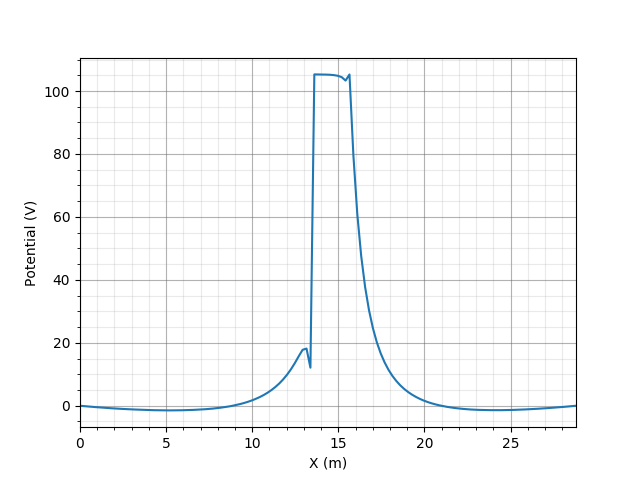
\includegraphics[width=\textwidth]{figures/MMO/BField/WB/L_BField_WB.png}
  \caption{Booms}
  \label{fig:L_BField_WB}
\end{subfigure}
\begin{subfigure}[b]{0.6\textwidth}
  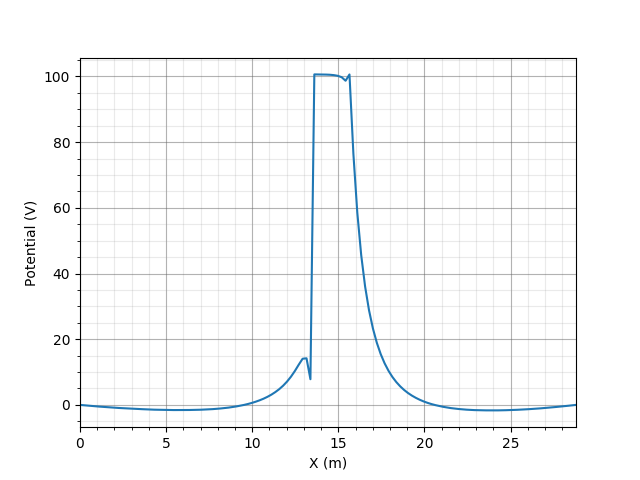
\includegraphics[width=\textwidth]{figures/MMO/BField/NB/L_BField_NB.png}
  \caption{Without booms}
  \label{fig:L_BField_NB}
\end{subfigure}
\label{fig:Line_BField}
\caption{Potential profile along the X axis for the two MMO configurations with drift along the negative Z axis, photoemission and an external magnetic field are included. The line is plotted at $(x,y) = (13.95 m, 13.95 m)$, or node points $(x,y) = (62,62)$, and passes through the main octagonal body of the spacecraft. The X axis units are in number of nodes from the origin. The two values in each plot show the height of the potential barrier formed.}
\end{figure}

%AVERAGE POTENTIAL ISOLINES XY
\begin{figure}[H]
  \begin{subfigure}[b]{0.6\textwidth}
    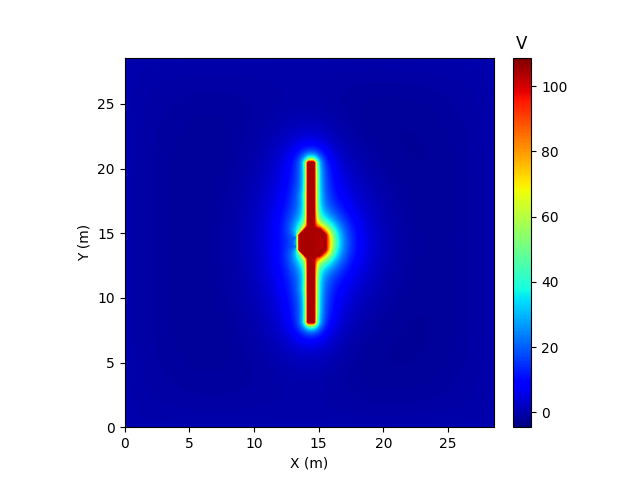
\includegraphics[width=\textwidth]{figures/MMO/BField/WB/P_BField_WB.png}
    \caption{Booms}
    \label{fig:P_BField_WB}
  \end{subfigure}
  \hfill
  \begin{subfigure}[b]{0.6\textwidth}
    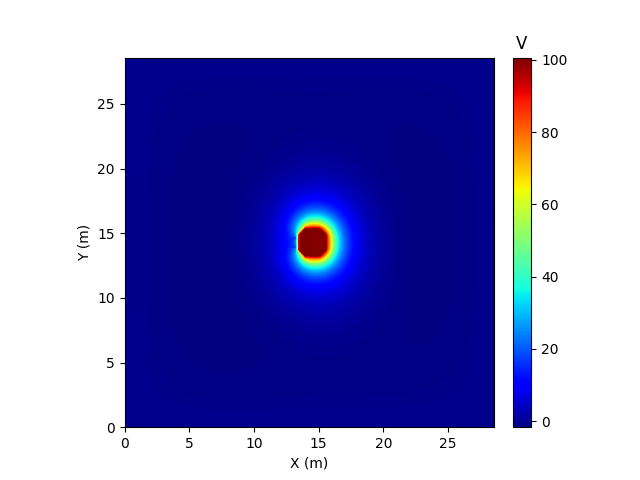
\includegraphics[width=\textwidth]{figures/MMO/BField/NB/P_BField_NB.png}
    \caption{Without booms}
    \label{fig:P_BField_NB}
  \end{subfigure}
  \label{fig:Pot_BField}
  \caption{2D slice through $Z = 14.4 m$ showing the time averaged potential profile of the entire computational domain with drift along the negative Z axis, photoemission and an external magnetic field are included. The potential is time averaged after a floating potential has been reached after 1,000 timesteps.}
\end{figure}

%PARTICLE DENSITIES (rho_i and rho_e)
%RHO_I
\begin{figure}[H]
  \begin{subfigure}[b]{0.6\textwidth}
  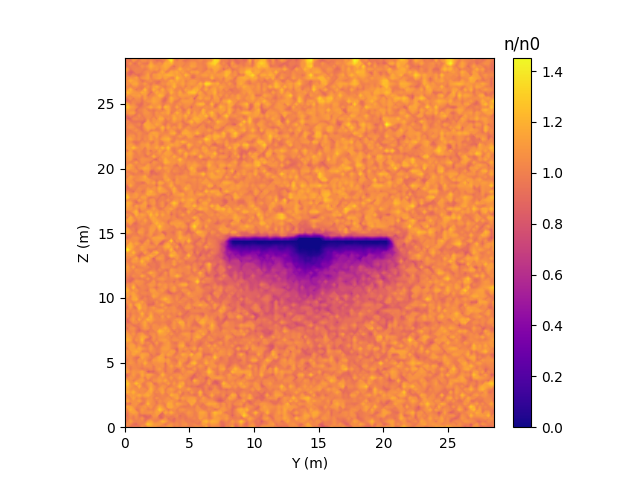
\includegraphics[width=\textwidth]{figures/MMO/BField/WB/I_BField_WB.png}
  \caption{Booms}
  \label{fig:I_BField_WB}
\end{subfigure}
\begin{subfigure}[b]{0.6\textwidth}
  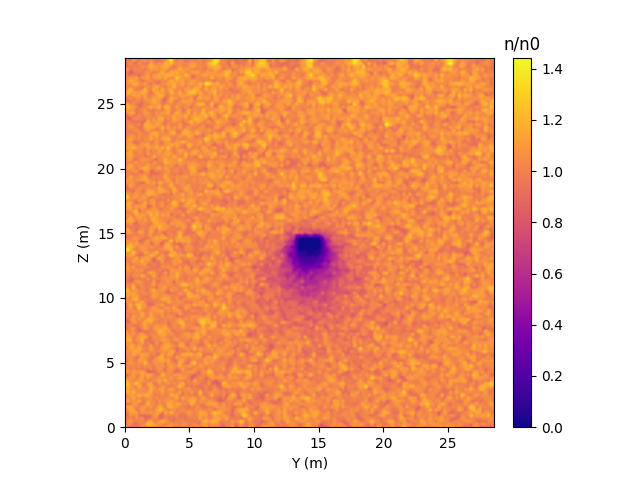
\includegraphics[width=\textwidth]{figures/MMO/BField/NB/I_BField_NB.png}
  \caption{Without booms}
  \label{fig:I_BField_NB}
\end{subfigure}
\label{fig:Ions_BField}
\caption{Ion density profile plotted at $Z = 14.4 m$, the color gradient is normalized against the ion plasma density from table \ref{tab:PlasmaParamMMO}. Drift is along the negative Z axis, photoemission and an external magnetic field are included.}
\end{figure}

%RHO_E
\begin{figure}[H]
  \begin{subfigure}[b]{0.6\textwidth}
  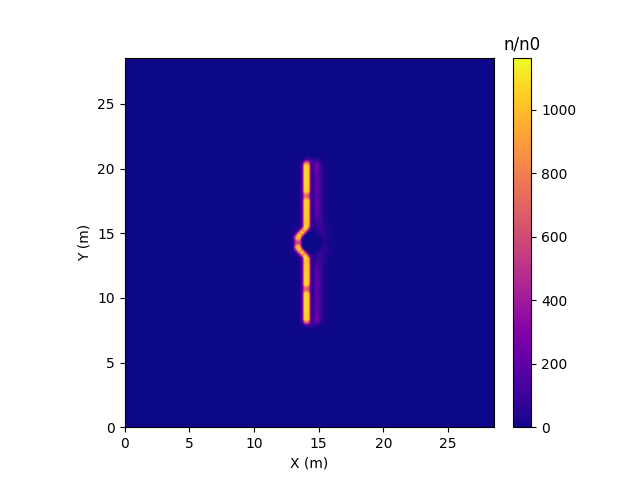
\includegraphics[width=\textwidth]{figures/MMO/BField/WB/E_BField_WB.png}
  \caption{Booms}
  \label{fig:E_BField_WB}
\end{subfigure}
\begin{subfigure}[b]{0.6\textwidth}
  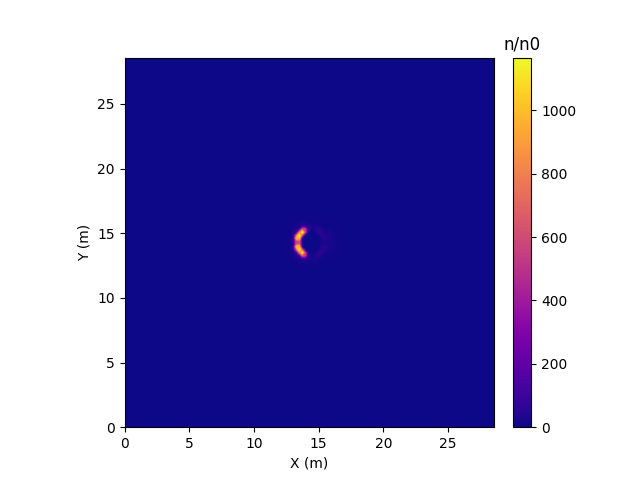
\includegraphics[width=\textwidth]{figures/MMO/BField/NB/E_BField_NB.png}
  \caption{Without booms}
  \label{fig:E_BField_NB}
\end{subfigure}
\label{fig:Elec_BField}
\caption{Electron density profile plotted at $Z = 14.4 m$, the color gradient is normalized against the electron plasma density from table \ref{tab:PlasmaParamMMO}.Drift is along the negative Z axis, photoemission and an external magnetic field are included. The direction of the sun is along the negative X axis.}
\end{figure}

\section{Charging at different photoelectron temperatures}

%FLOATING POTENTIAL CONVERGENCE
\begin{figure}[H]
  \centering
  \begin{subfigure}[b]{0.75\textwidth}
  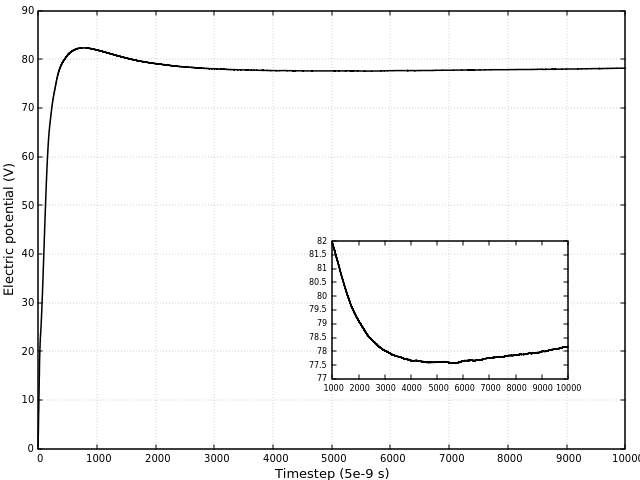
\includegraphics[width=\columnwidth]{figures/MMO/PHTemp/WB/C_PHTemp_WB.png}
  \caption{Booms}
  \label{fig:C_PHTemp_WB}
\end{subfigure}
\par\bigskip
\begin{subfigure}[b]{0.75\textwidth}
  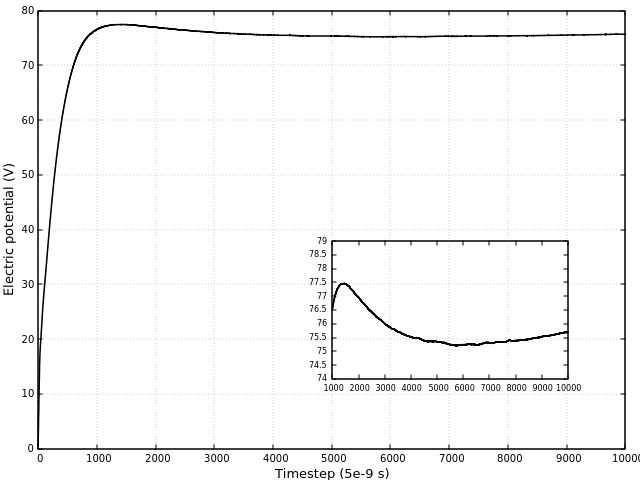
\includegraphics[width=\columnwidth]{figures/MMO/PHTemp/NB/C_PHTemp_NB.png}
  \caption{Without booms}
  \label{fig:C_PHTemp_NB}
\end{subfigure}
\label{fig:Conv_PHTemp}
\caption{Timeseries plot of the potential of the two configurations of the MMO, drift is along the negative Z axis and the photoelectron temperature has been set to $3 \; eV$. The potential has been converted from PINC dimensionless units to Volts. The inset plots the same timeseries after 1000 timesteps, where the potential of the spacecraft has begun to oscillate about the floating potential.}
\end{figure}

%POTENTIAL THROUGH CENTER OF OBJECT
\begin{figure}[H]
  \begin{subfigure}[b]{0.6\textwidth}
  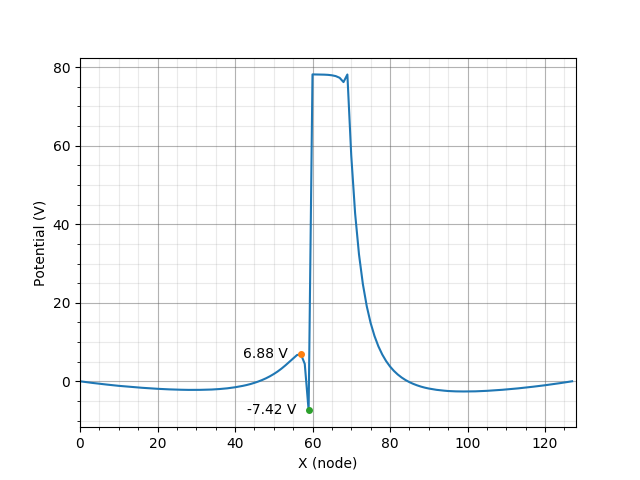
\includegraphics[width=\textwidth]{figures/MMO/PHTemp/WB/L_PHTemp_WB.png}
  \caption{Booms}
  \label{fig:L_PHTemp_WB}
\end{subfigure}
\begin{subfigure}[b]{0.6\textwidth}
  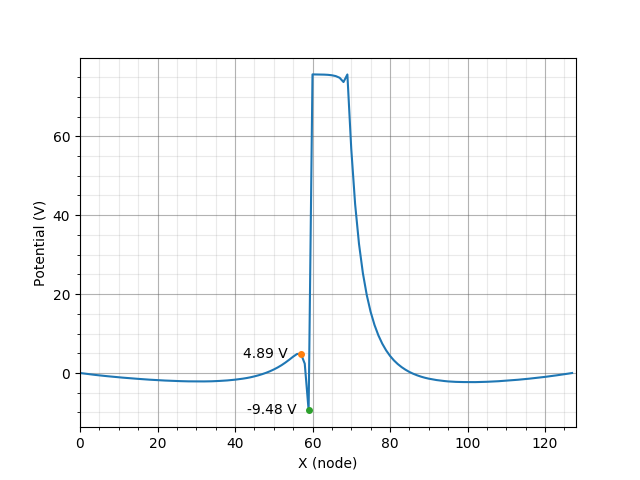
\includegraphics[width=\textwidth]{figures/MMO/PHTemp/NB/L_PHTemp_NB.png}
  \caption{Without booms}
  \label{fig:L_PHTemp_NB}
\end{subfigure}
\label{fig:Line_PHTemp}
\caption{Potential profile along the X axis for the two MMO configurations with drift along the negative Z axis, photoemission is included with a photoelectron temperature of $3 \; eV$. The line is plotted at $(x,y) = (13.95 m, 13.95 m)$, or node points $(x,y) = (62,62)$, and passes through the main octagonal body of the spacecraft. The X axis units are in number of nodes from the origin. The two values in each plot show the height of the potential barrier formed.}
\end{figure}

%AVERAGE POTENTIAL ISOLINES XY
\begin{figure}[H]
  \begin{subfigure}[b]{0.6\textwidth}
    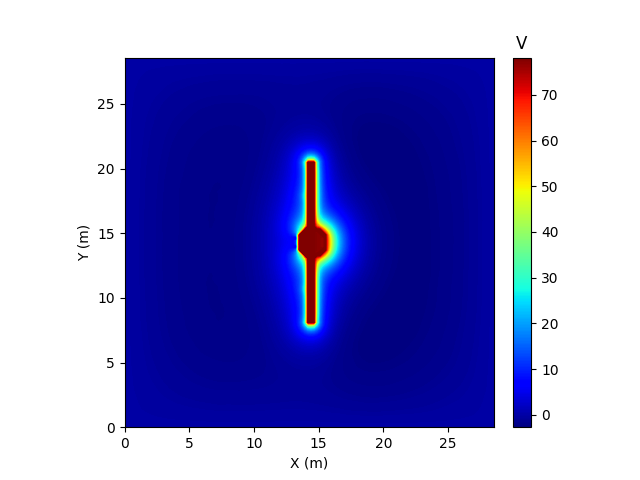
\includegraphics[width=\textwidth]{figures/MMO/PHTemp/WB/P_PHTemp_WB.png}
    \caption{Booms}
    \label{fig:P_PHTemp_WB}
  \end{subfigure}
  \hfill
  \begin{subfigure}[b]{0.6\textwidth}
    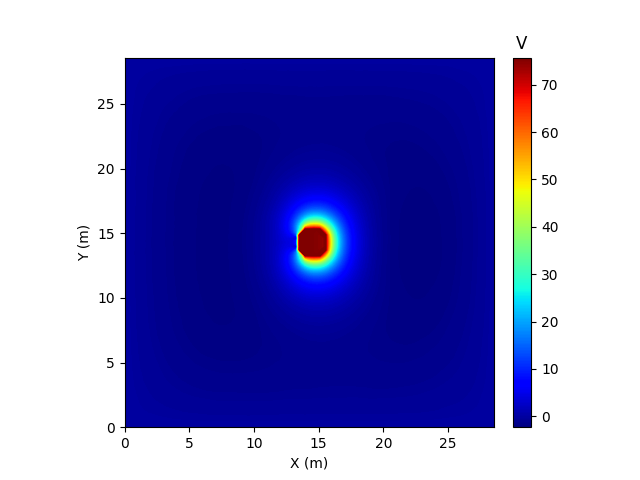
\includegraphics[width=\textwidth]{figures/MMO/PHTemp/NB/P_PHTemp_NB.png}
    \caption{Without booms}
    \label{fig:P_PHTemp_NB}
  \end{subfigure}
  \label{fig:Pot_PHTemp}
  \caption{2D cut through $Z = 14.4 m$ showing the time averaged potential profile of the entire computational domain with drift along the negative Z axis, photoemission is included with a photoelectron temperature of $3 \; eV$. The potential is time averaged after a floating potential has been reached after 1,000 timesteps.}
\end{figure}

%PARTICLE DENSITIES (rho_i and rho_e)
%RHO_I
\begin{figure}[H]
  \begin{subfigure}[b]{0.6\textwidth}
  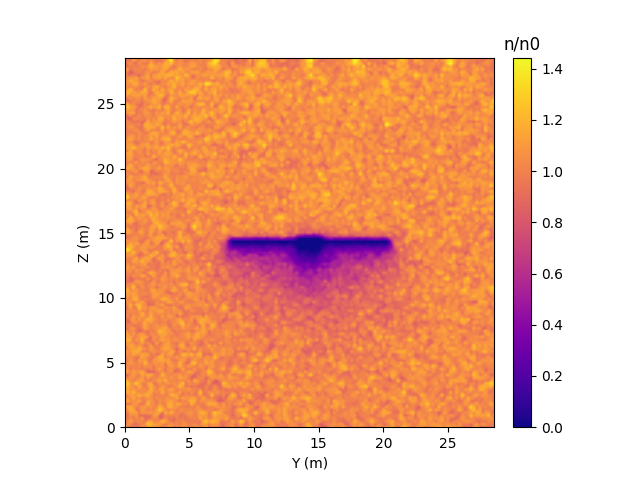
\includegraphics[width=\textwidth]{figures/MMO/PHTemp/WB/I_PHTemp_WB.png}
  \caption{Booms}
  \label{fig:I_PHTemp_WB}
\end{subfigure}
\begin{subfigure}[b]{0.6\textwidth}
  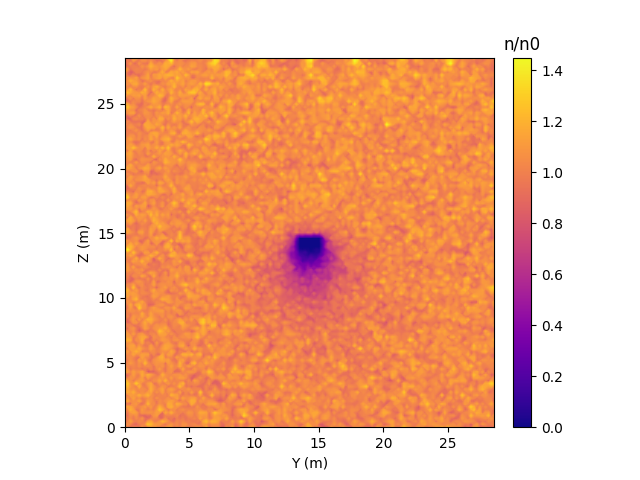
\includegraphics[width=\textwidth]{figures/MMO/PHTemp/NB/I_PHTemp_NB.png}
  \caption{Without booms}
  \label{fig:I_PHTemp_NB}
\end{subfigure}
\label{fig:Ions_PHTemp}
\caption{Ion density profile plotted at $Z = 14.4 m$, the color gradient is normalized against the ion plasma density from table \ref{tab:PlasmaParamMMO}. Drift is along the negative Z axis, and photoemission is included with a photoelectron temperature of $3 \; eV$.}
\end{figure}

%RHO_E
\begin{figure}[H]
  \begin{subfigure}[b]{0.6\textwidth}
  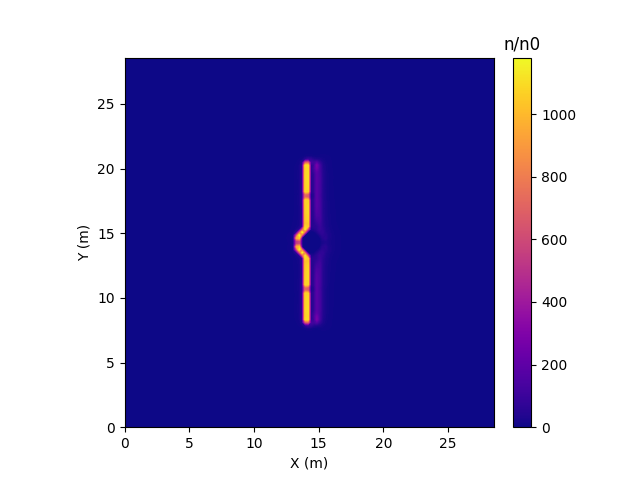
\includegraphics[width=\textwidth]{figures/MMO/PHTemp/WB/E_PHTemp_WB.png}
  \caption{Booms}
  \label{fig:E_PHTemp_WB}
\end{subfigure}
\begin{subfigure}[b]{0.6\textwidth}
  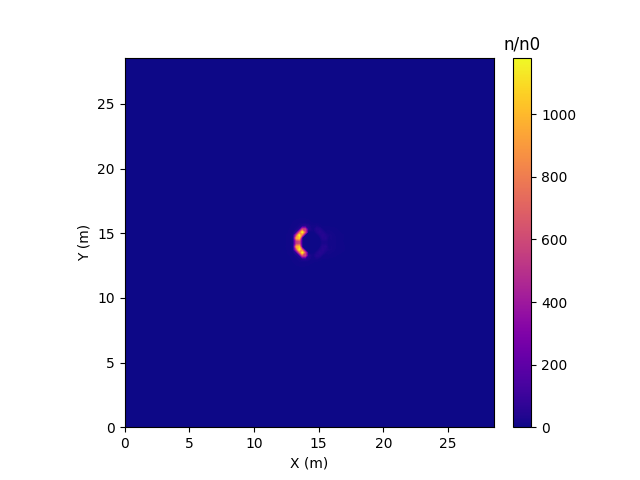
\includegraphics[width=\textwidth]{figures/MMO/PHTemp/NB/E_PHTemp_NB.png}
  \caption{Without booms}
  \label{fig:E_PHTemp_NB}
\end{subfigure}
\label{fig:Elec_PHTemp}
\caption{Electron density profile plotted at $Z = 14.4 m$, the color gradient is normalized against the electron plasma density from table \ref{tab:PlasmaParamMMO}. Drift is along the negative Z axis, and photoemission is included with a photoelectron temperature of $3 \; eV$.}
\end{figure}